\begin{figure}[ht!]
\centering
% manually adjust the width of the figure
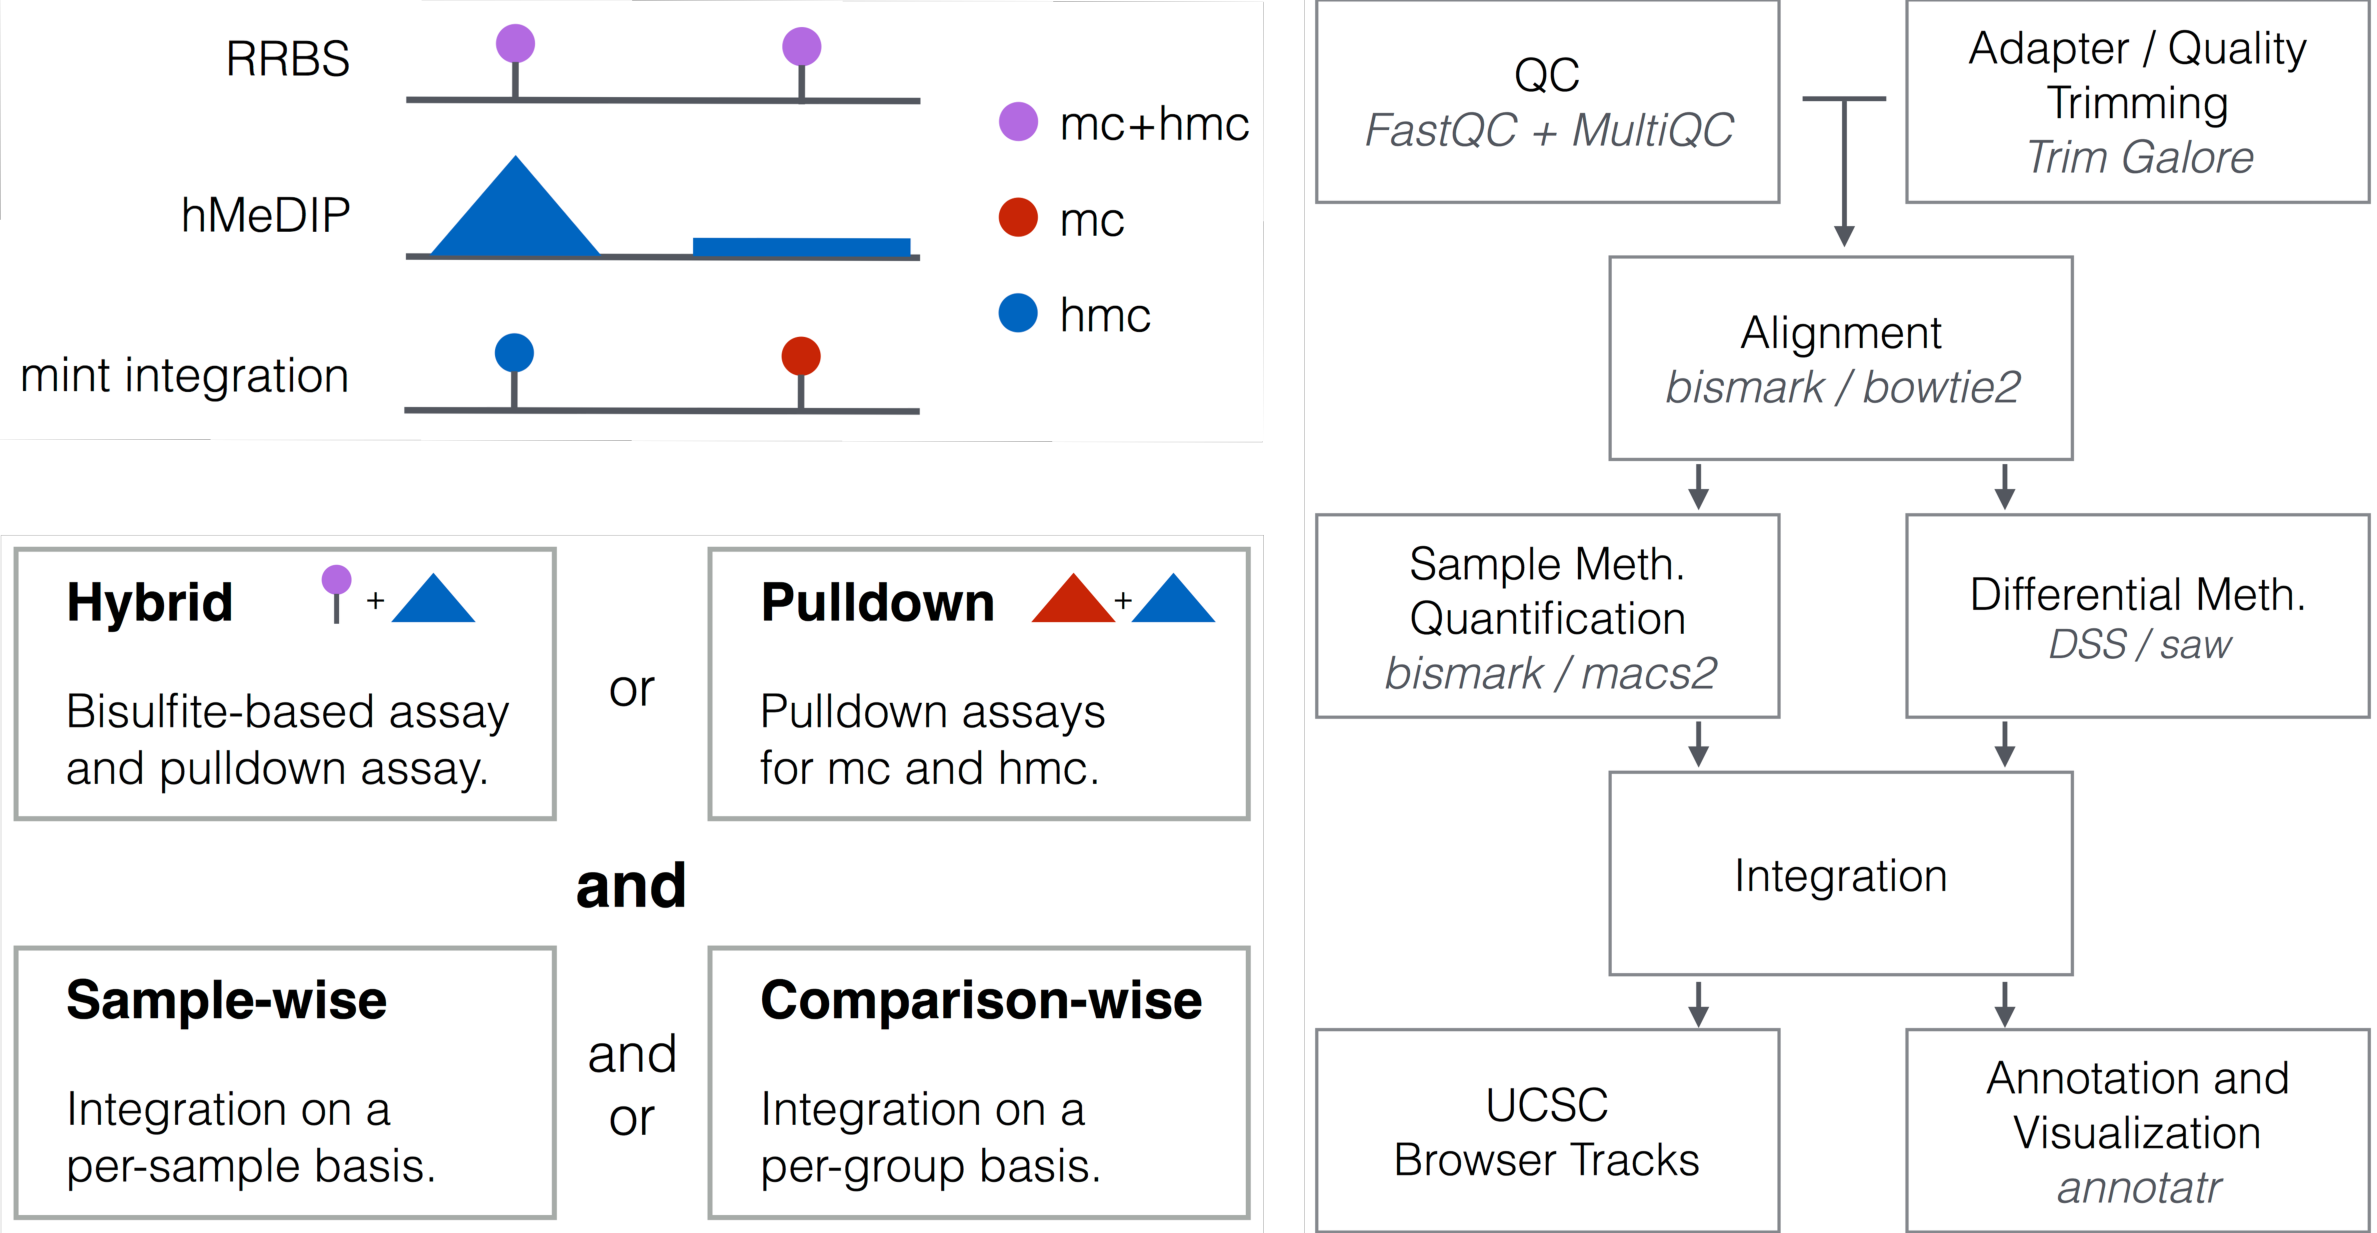
\includegraphics[width=1\textwidth]{chap5figs/figure5_1.pdf}
\caption[Conceptual overview of mint and implementation.]
{
% Rackham requires the figure list title matches the first sentence, so repeat that sentence here
\textbf{Conceptual overview of mint and implementation.} The concept behind 5mC and 5hmC integration. A summary of supported experimental setups and analyses. The overall mint workflow, with the primary tools used in each module.
}
\label{chap5:fig:1}
\end{figure}

\newpage

\begin{figure}[ht!]
\centering
% manually adjust the width of the figure
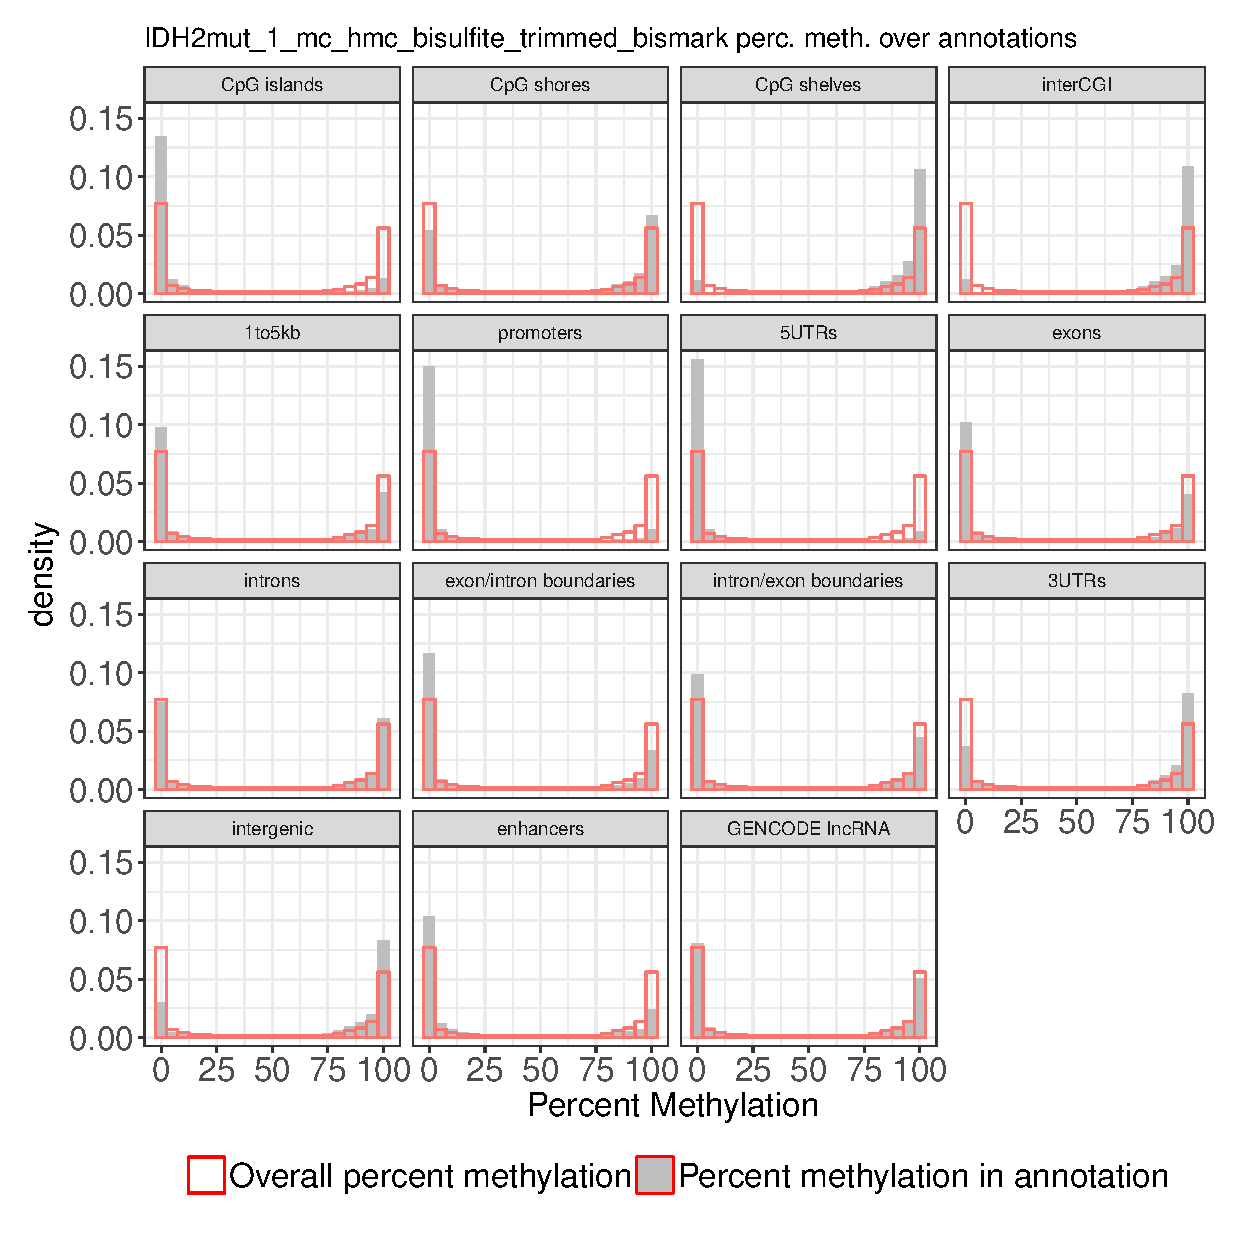
\includegraphics[width=1\textwidth]{chap5figs/figure5_2.eps}
\caption[The percent methylation in annotations from sample RRBS data.]
{
% Rackham requires the figure list title matches the first sentence, so repeat that sentence here
\textbf{The percent methylation in annotations from sample RRBS data.}
}
\label{chap5:fig:2}
\end{figure}

\newpage

\begin{figure}[ht!]
\centering
% manually adjust the width of the figure
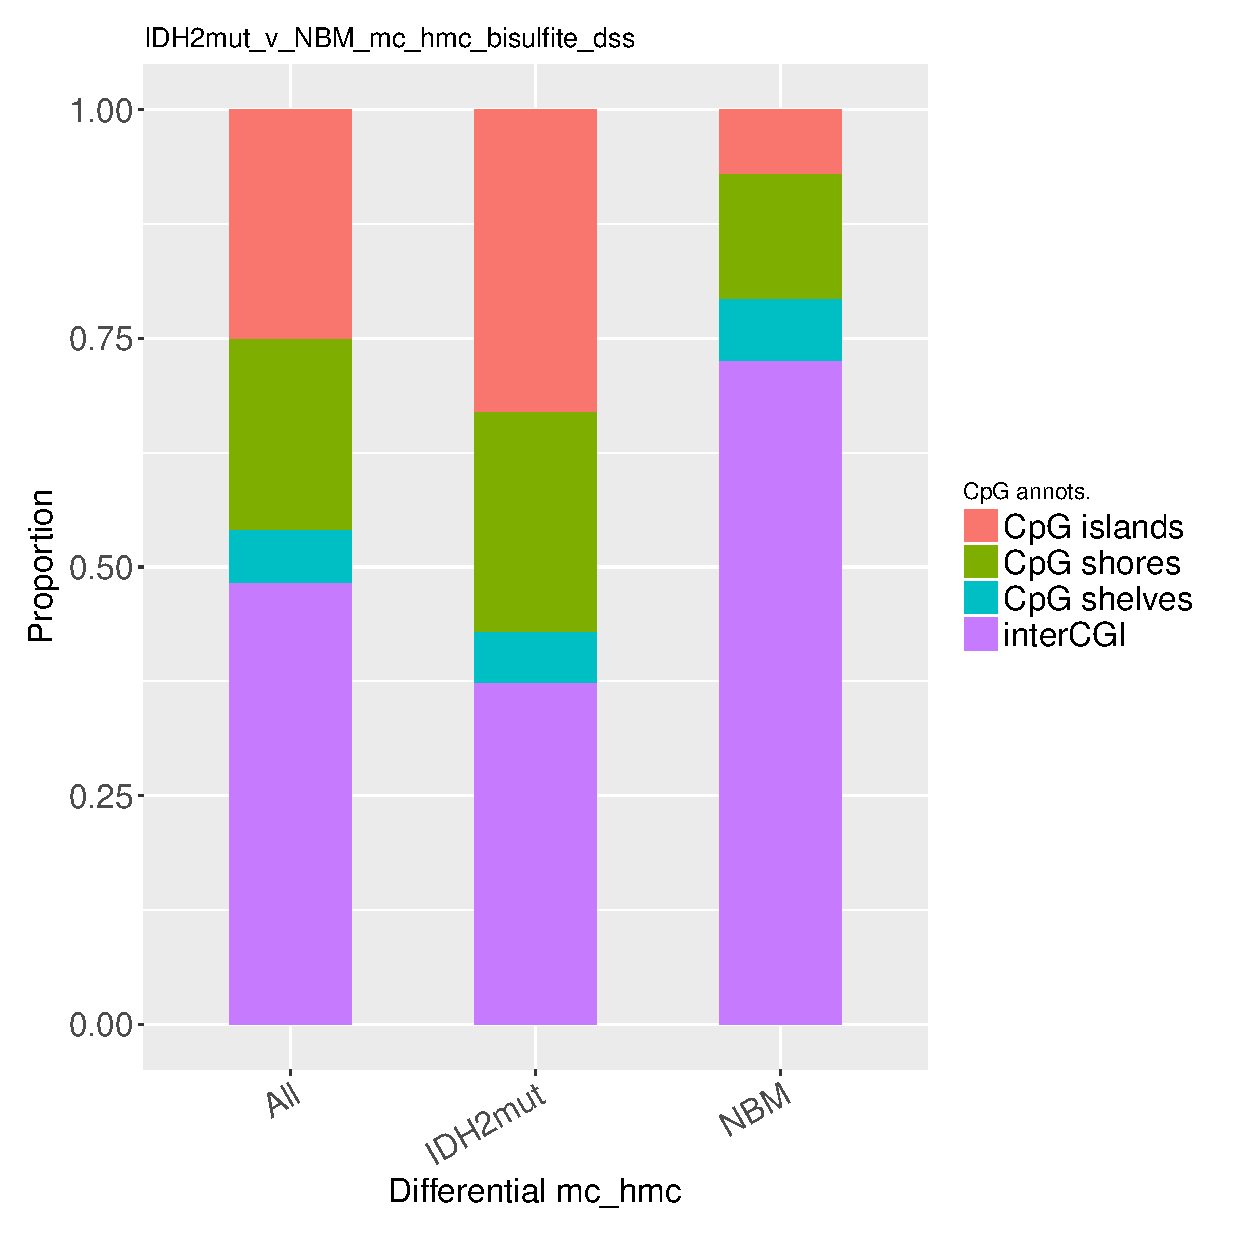
\includegraphics[width=1\textwidth]{chap5figs/figure5_3.eps}
\caption[The distribution of DhMRs from hMeSeal in CpG features.]
{
% Rackham requires the figure list title matches the first sentence, so repeat that sentence here
\textbf{The distribution of DhMRs from hMeSeal in CpG features.}
}
\label{chap5:fig:3}
\end{figure}

\newpage

\begin{figure}[ht!]
\centering
% manually adjust the width of the figure
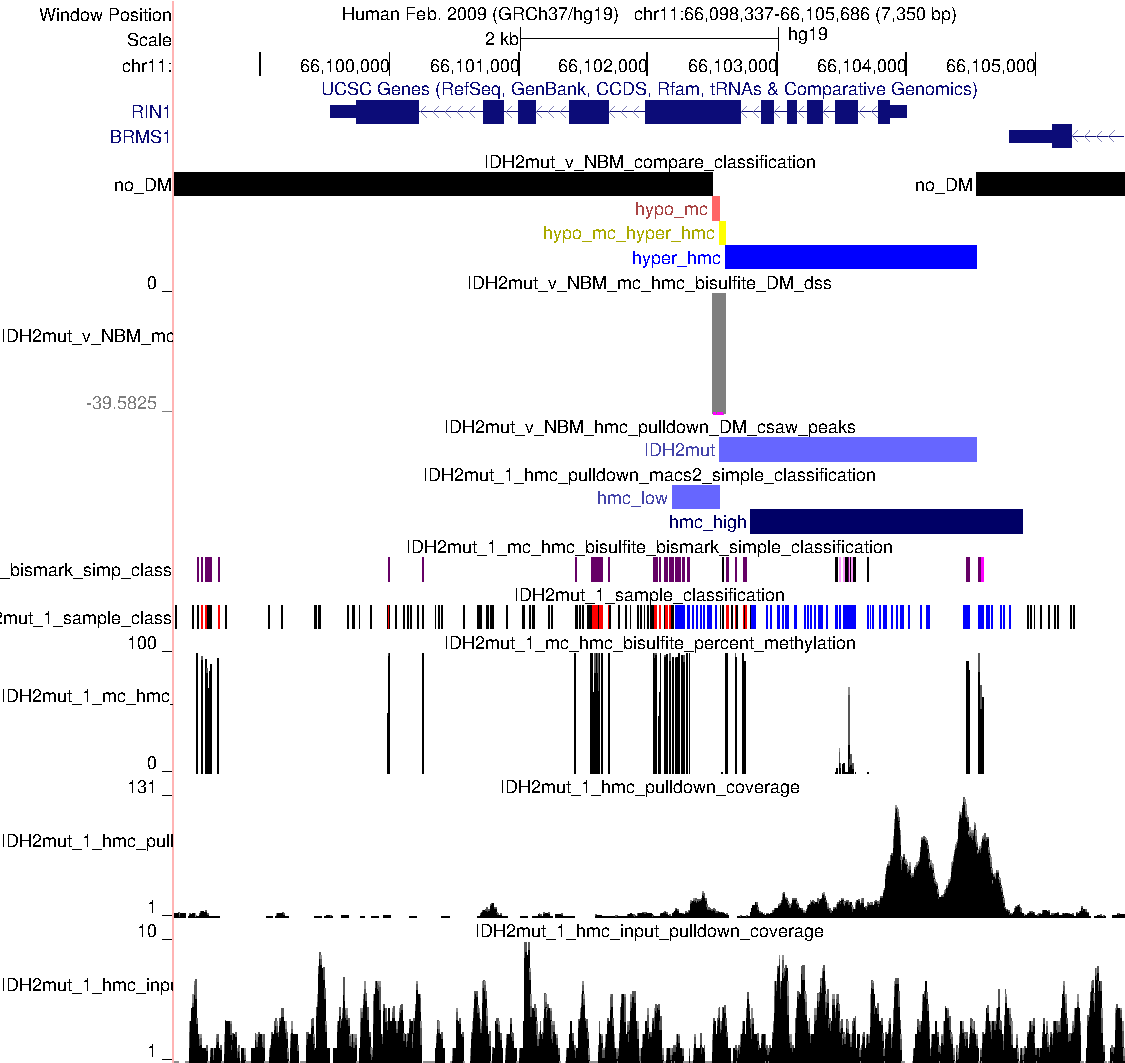
\includegraphics[width=1\textwidth]{chap5figs/figure5_4.pdf}
\caption[Example of UCSC Genome Browser tracks.]
{
% Rackham requires the figure list title matches the first sentence, so repeat that sentence here
\textbf{Example of UCSC Genome Browser tracks.} The RIN1 locus showing coordinated hypo 5mC and hyper 5hmC (yellow) in an internal exon and hyper 5hmC at the 5' end (blue).
}
\label{chap5:fig:4}
\end{figure}

\newpage

\begin{figure}[ht!]
\centering
% manually adjust the width of the figure
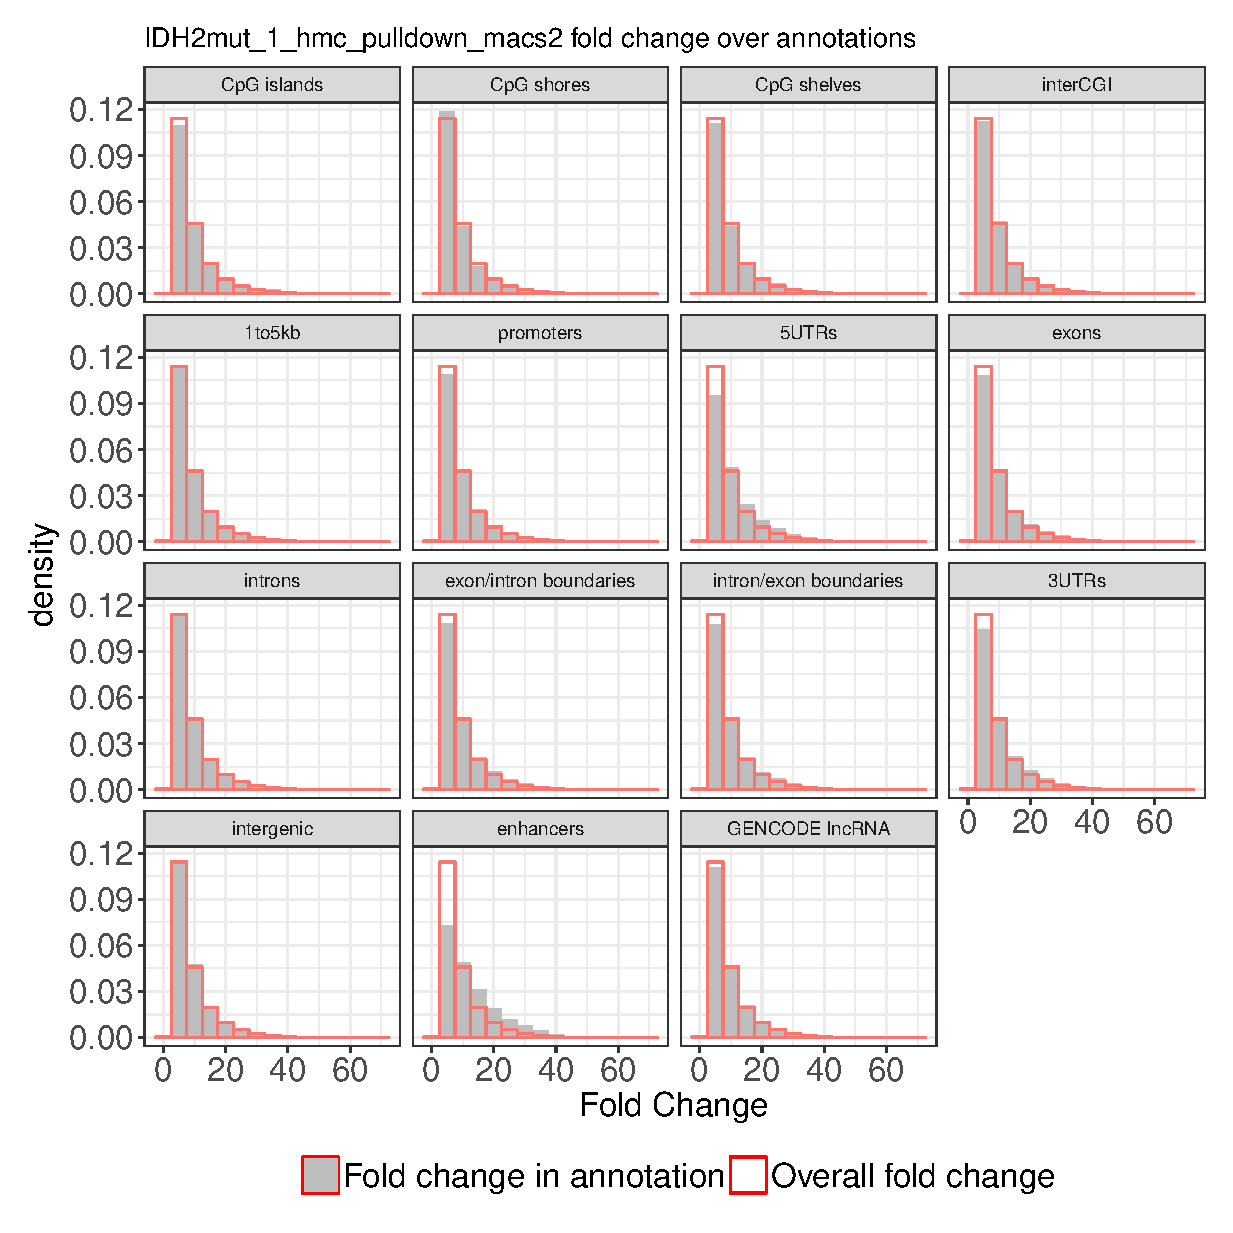
\includegraphics[width=1\textwidth]{chap5figs/figure5_5.eps}
\caption[Fold change of macs2 peaks measuring hydroxymethylation across genomic annotations.]
{
% Rackham requires the figure list title matches the first sentence, so repeat that sentence here
\textbf{Fold change of macs2 peaks measuring hydroxymethylation across genomic annotations.} Gray bars denote the fold change distribution for peaks annotated to the feature labeling the facet, and red outlines are the overall distribution of peak fold changes. Of note is the hyper-hydroxymethylation present in peaks annotated to enhancers and 5'UTRs compared to background.
}
\label{chap5:fig:5}
\end{figure}

\newpage

\begin{figure}[ht!]
\centering
% manually adjust the width of the figure
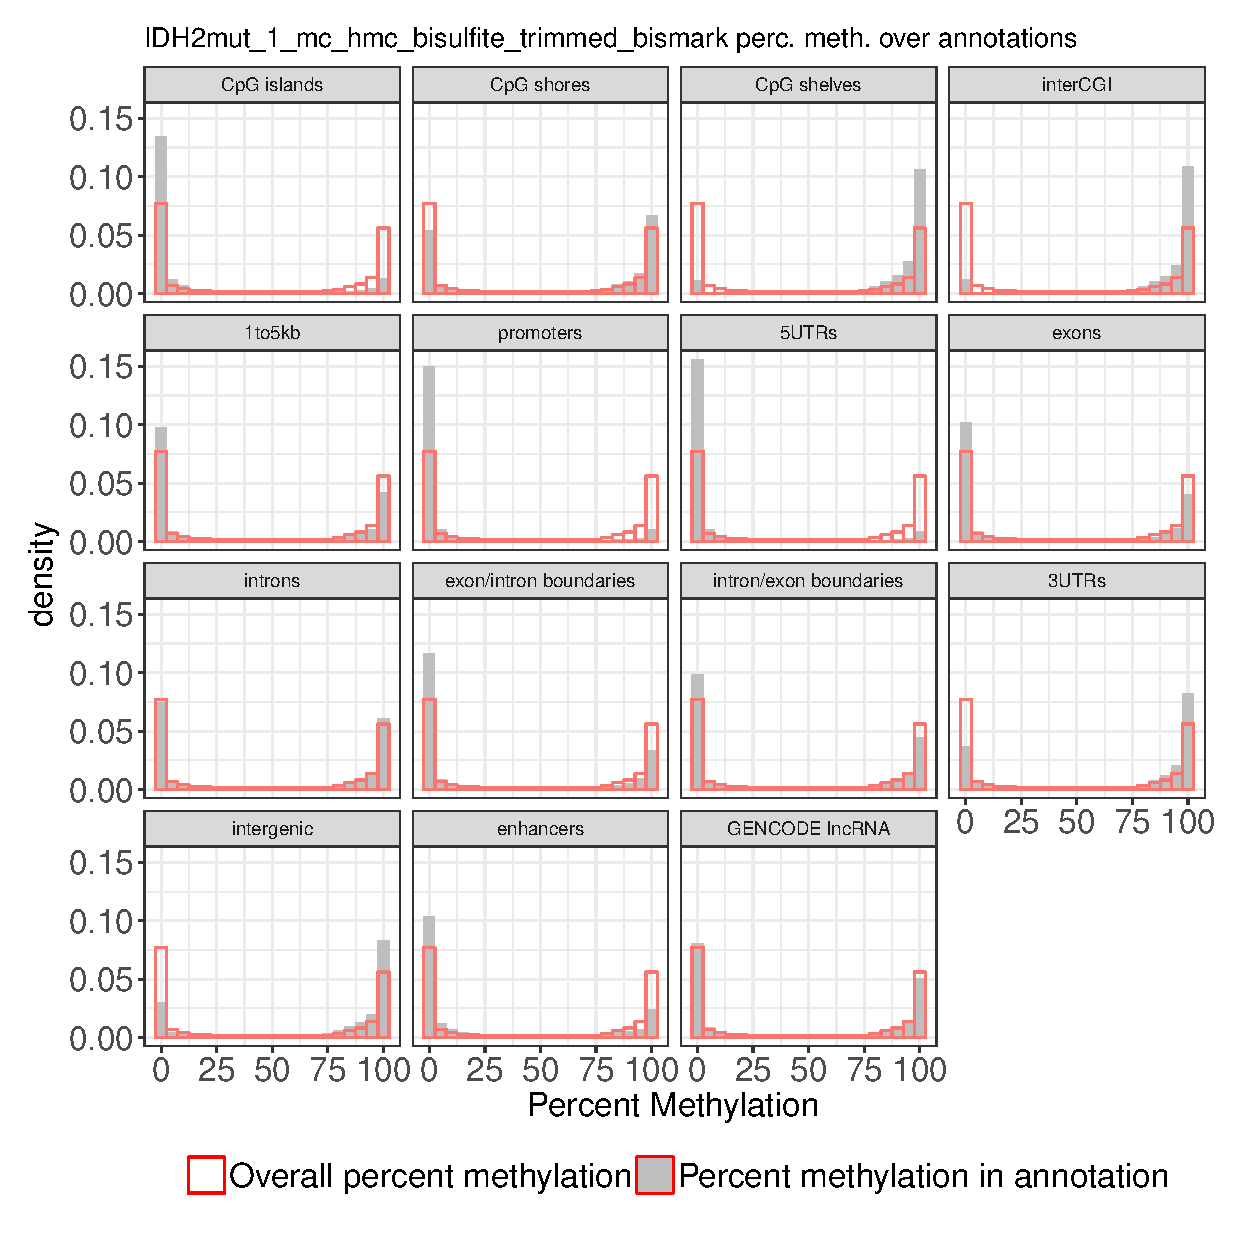
\includegraphics[width=1\textwidth]{chap5figs/figure5_6.eps}
\caption[Percent methylation of CpGs across genomic annotations.]
{
% Rackham requires the figure list title matches the first sentence, so repeat that sentence here
\textbf{Percent methylation of CpGs across genomic annotations.} Gray bars and red outlines are as in panel A. Of note is the hypo-methylation of CpGs annotated to enhancers and 5'UTRs relative to background, especially in light of corresponding hyper-hydroxymethylation.
}
\label{chap5:fig:6}
\end{figure}

\newpage

\begin{figure}[ht!]
\centering
% manually adjust the width of the figure
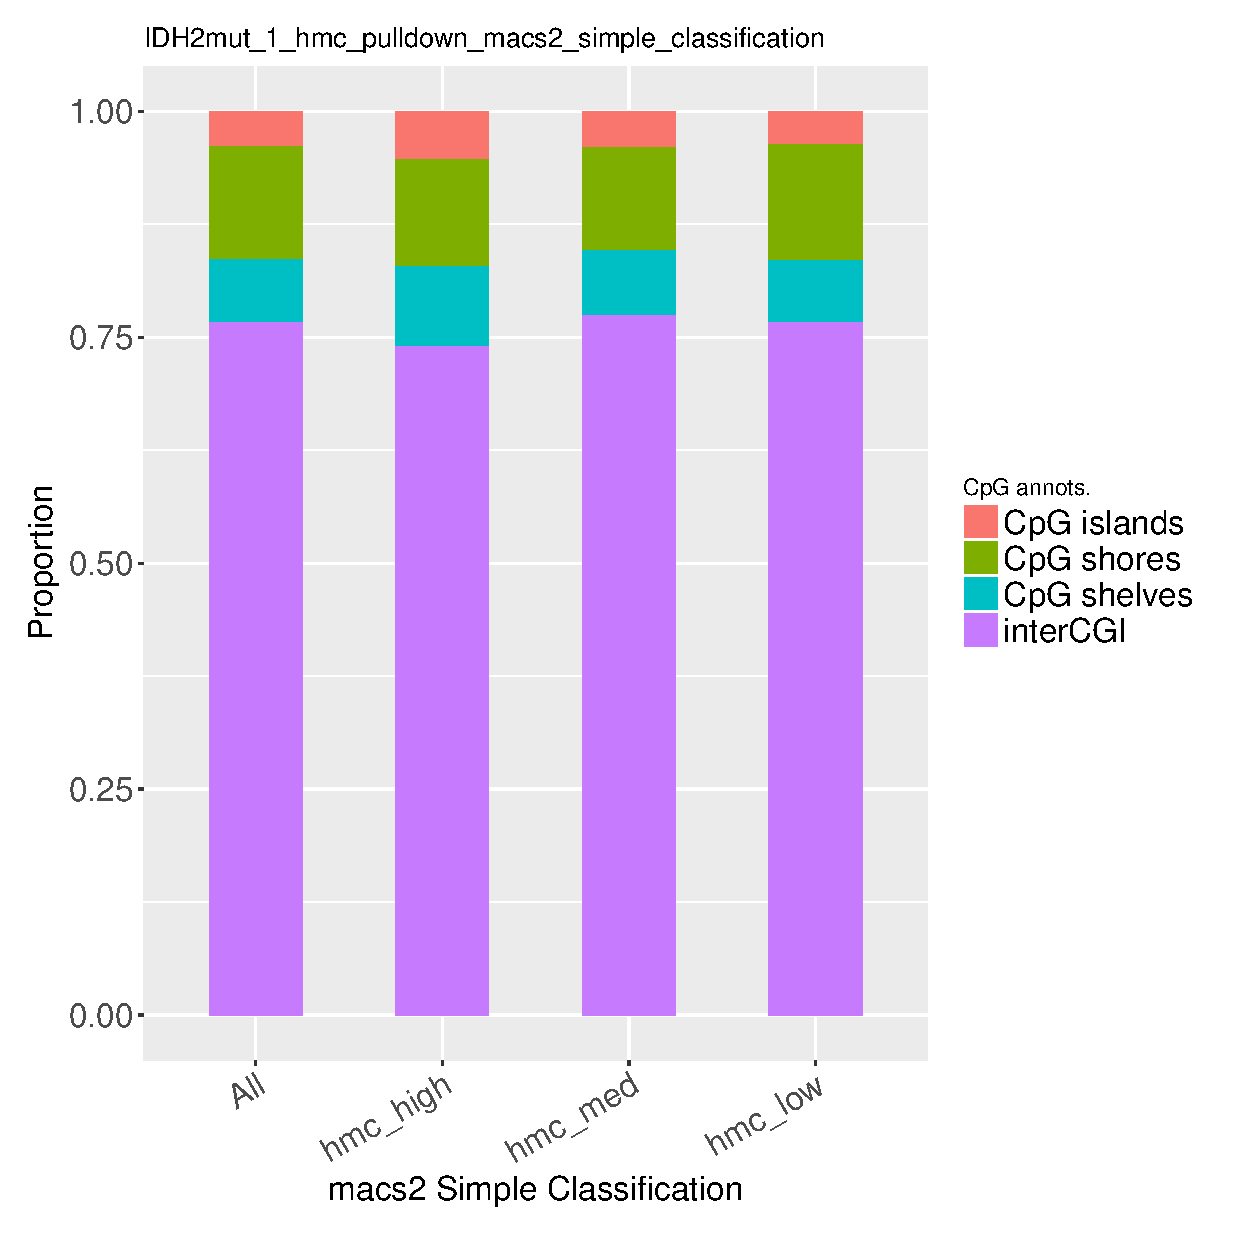
\includegraphics[width=1\textwidth]{chap5figs/figure5_7.eps}
\caption[Annotations of the simple classification across CpG features.]
{
% Rackham requires the figure list title matches the first sentence, so repeat that sentence here
\textbf{Annotations of the simple classification for hydroxymethylation across CpG features.} Classifications of hydroxymethylation are similarly distributed across CpG features regardless of peak strength.
}
\label{chap5:fig:7}
\end{figure}

\newpage

\begin{figure}[ht!]
\centering
% manually adjust the width of the figure
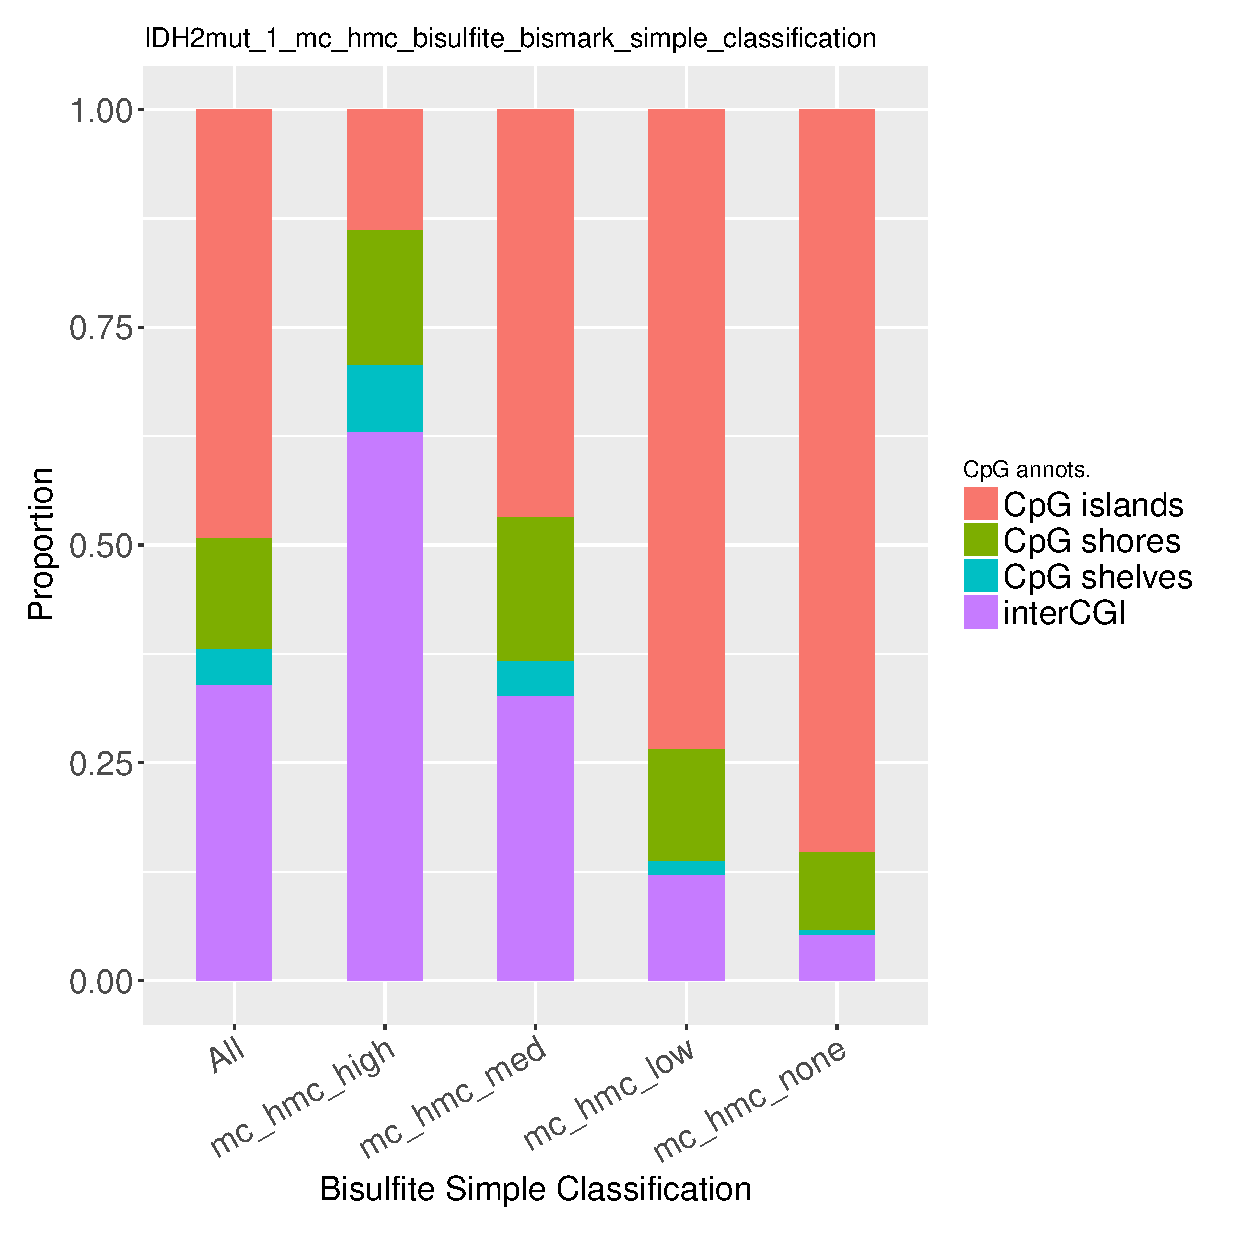
\includegraphics[width=1\textwidth]{chap5figs/figure5_8.eps}
\caption[Annotations of the simple classification.]
{
% Rackham requires the figure list title matches the first sentence, so repeat that sentence here
\textbf{Annotations of the simple classification for methylation across CpG features.} CpGs have different distributions across CpG features according to strength of methylation. In particular, as methylation weakens, it tends to be located more in CpG islands (orange), but less in CpG shelves (blue).
}
\label{chap5:fig:8}
\end{figure}

\newpage

\begin{figure}[ht!]
\centering
% manually adjust the width of the figure
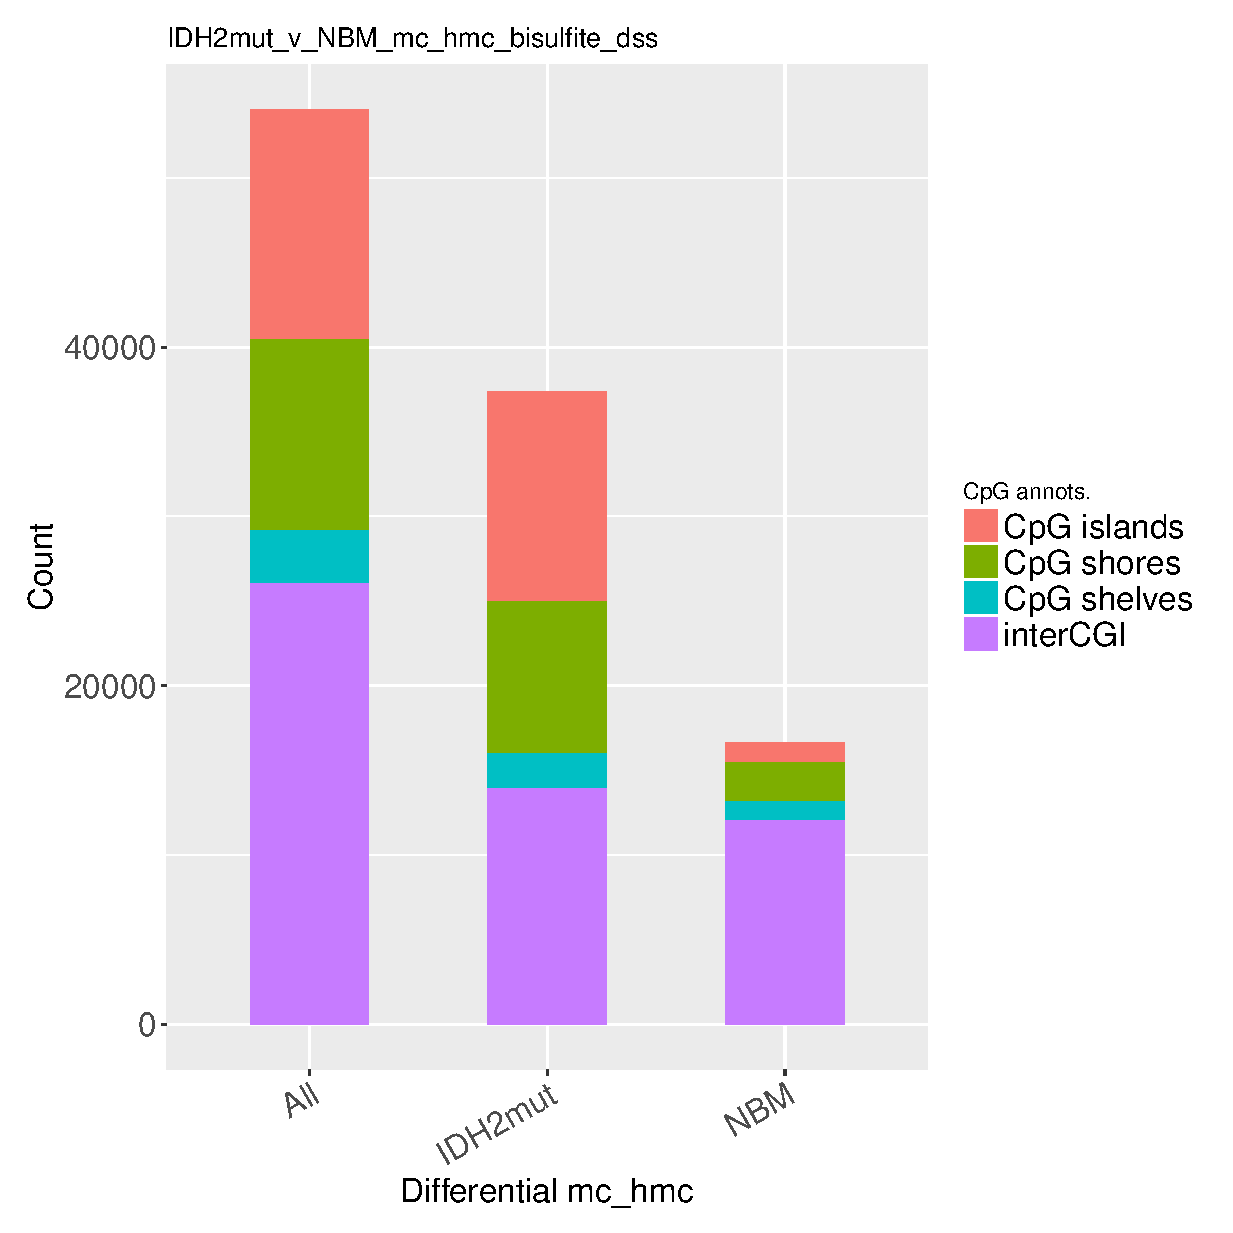
\includegraphics[width=1\textwidth]{chap5figs/figure5_9.eps}
\caption[Number of DMRs found by DSS, and annotated to CpG island features.]
{
% Rackham requires the figure list title matches the first sentence, so repeat that sentence here
\textbf{Number of DMRs found by DSS, and annotated to CpG island features.} The number of hyper-methylated DMRs in the IDH2 samples is greater than those in NBM samples, in line with previous findings.
}
\label{chap5:fig:9}
\end{figure}

\newpage

\begin{figure}[ht!]
\centering
% manually adjust the width of the figure
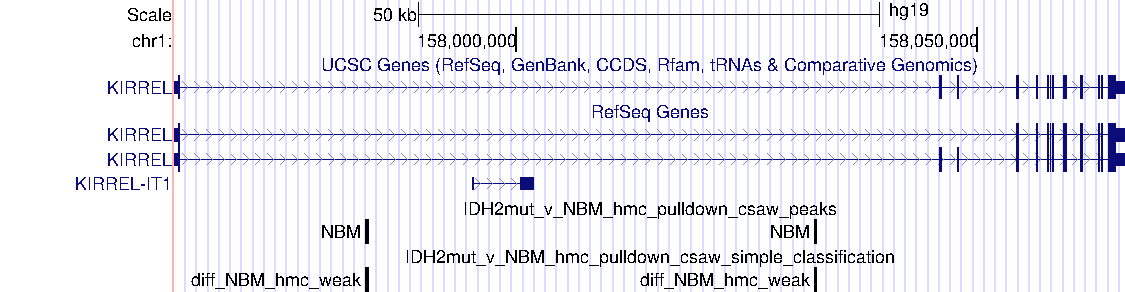
\includegraphics[width=1\textwidth]{chap5figs/figure5_10.pdf}
\caption[DhMRs at the KIRREL locus.]
{
% Rackham requires the figure list title matches the first sentence, so repeat that sentence here
\textbf{DhMRs at the KIRREL locus.} The Genome Browser with csaw track showing 'NBM' peaks (hypo-hydroxymethylated in IDH2 mutants) as was found in the paper originally describing the AML data.
}
\label{chap5:fig:10}
\end{figure}

\newpage

\begin{figure}[ht!]
\centering
% manually adjust the width of the figure
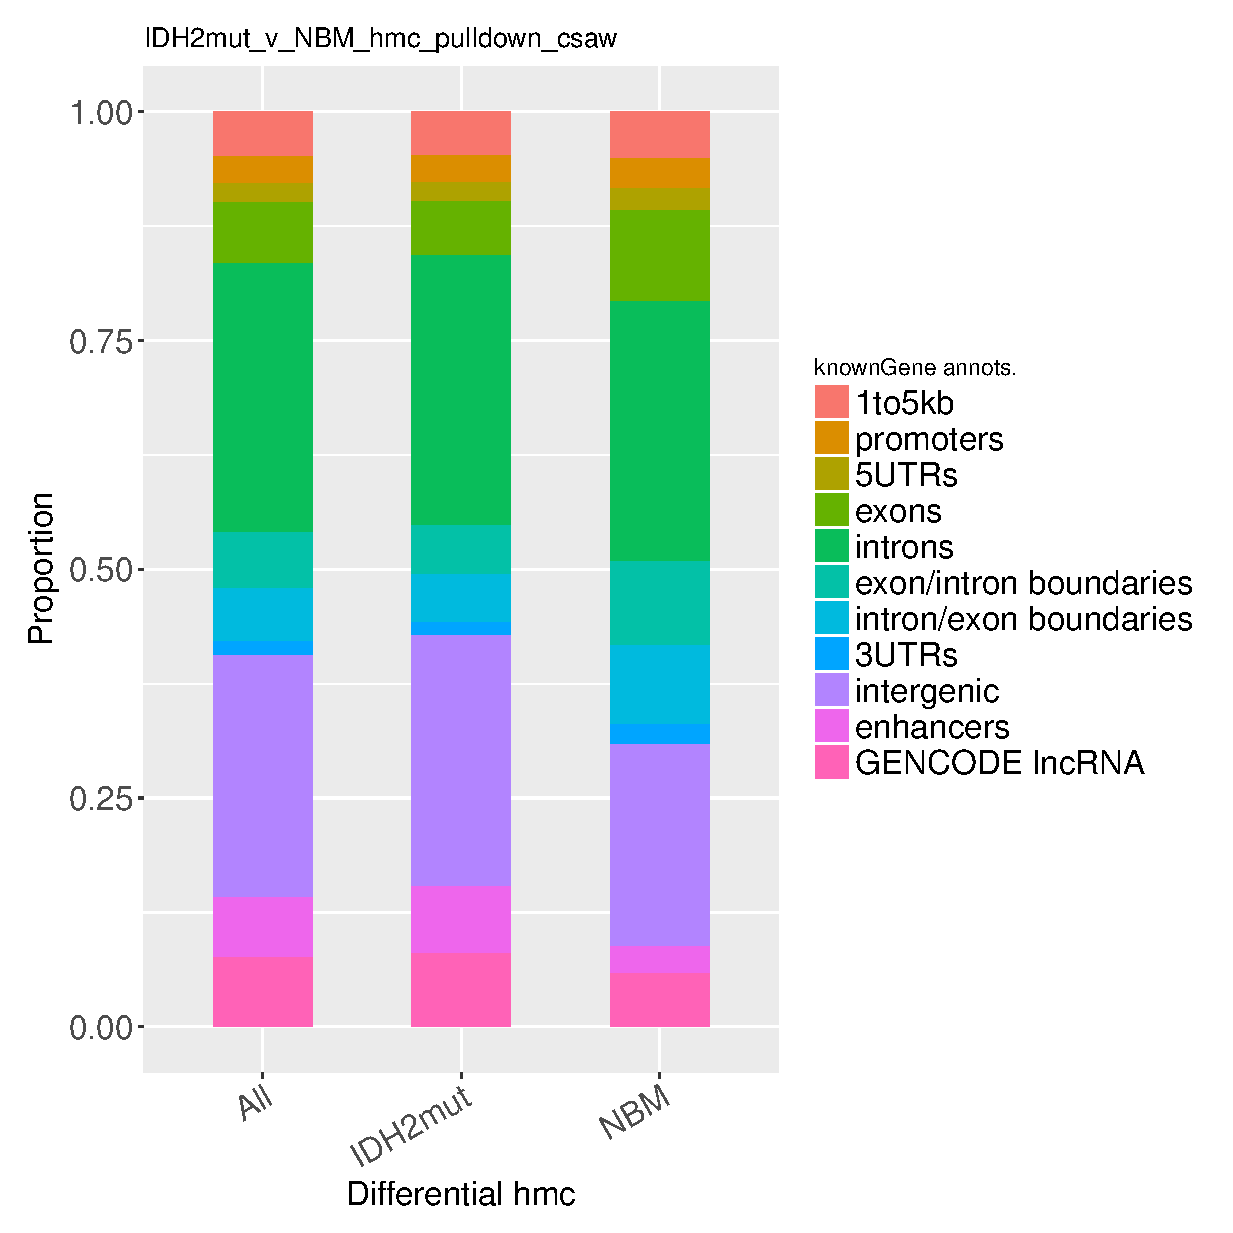
\includegraphics[width=1\textwidth]{chap5figs/figure5_11.eps}
\caption[DhMRs at genic annotations.]
{
% Rackham requires the figure list title matches the first sentence, so repeat that sentence here
\textbf{DhMRs at genic annotations.} Hypo-hydroxymethylated regions in IDH2 mutants occur more frequently at 5' ends of genes and exons than hyper-hydroxymethylated regions.
}
\label{chap5:fig:11}
\end{figure}

\newpage

\begin{figure}[ht!]
\centering
% manually adjust the width of the figure
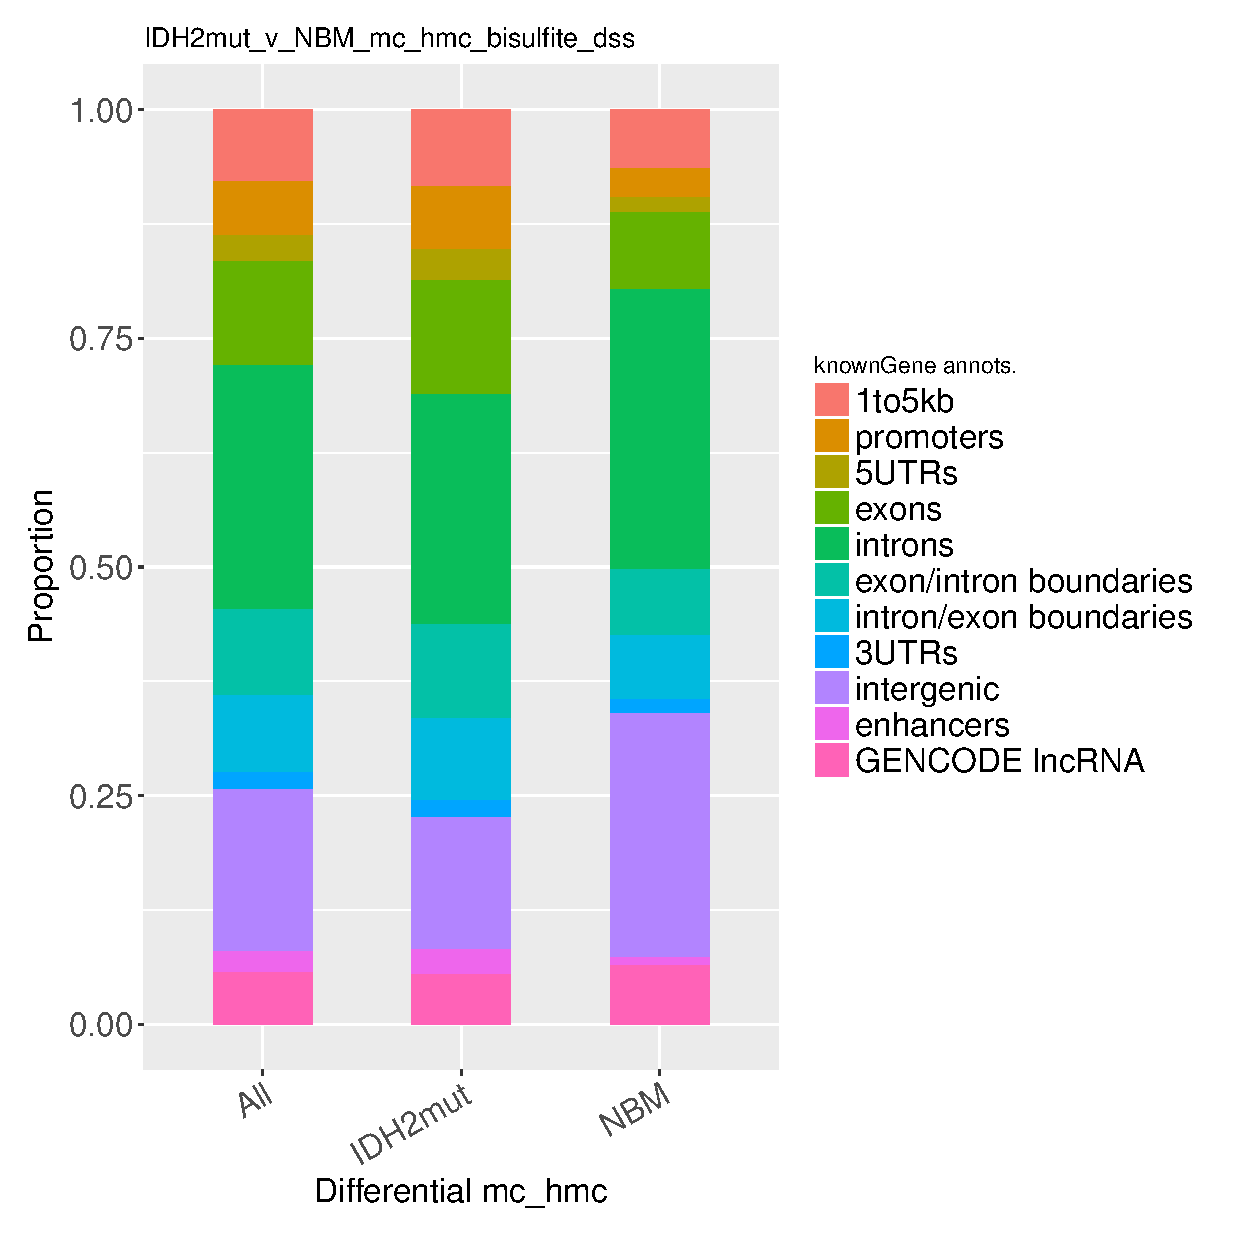
\includegraphics[width=1\textwidth]{chap5figs/figure5_12.eps}
\caption[DMRs at genic annotations.]
{
% Rackham requires the figure list title matches the first sentence, so repeat that sentence here
\textbf{DMRs at genic annotations.} Hyper-methylated regions in IDH2 mutants occur more frequently at 5' ends of genes and exons than hypo-methylated regions.
}
\label{chap5:fig:12}
\end{figure}

\newpage

\begin{figure}[ht!]
\centering
% manually adjust the width of the figure
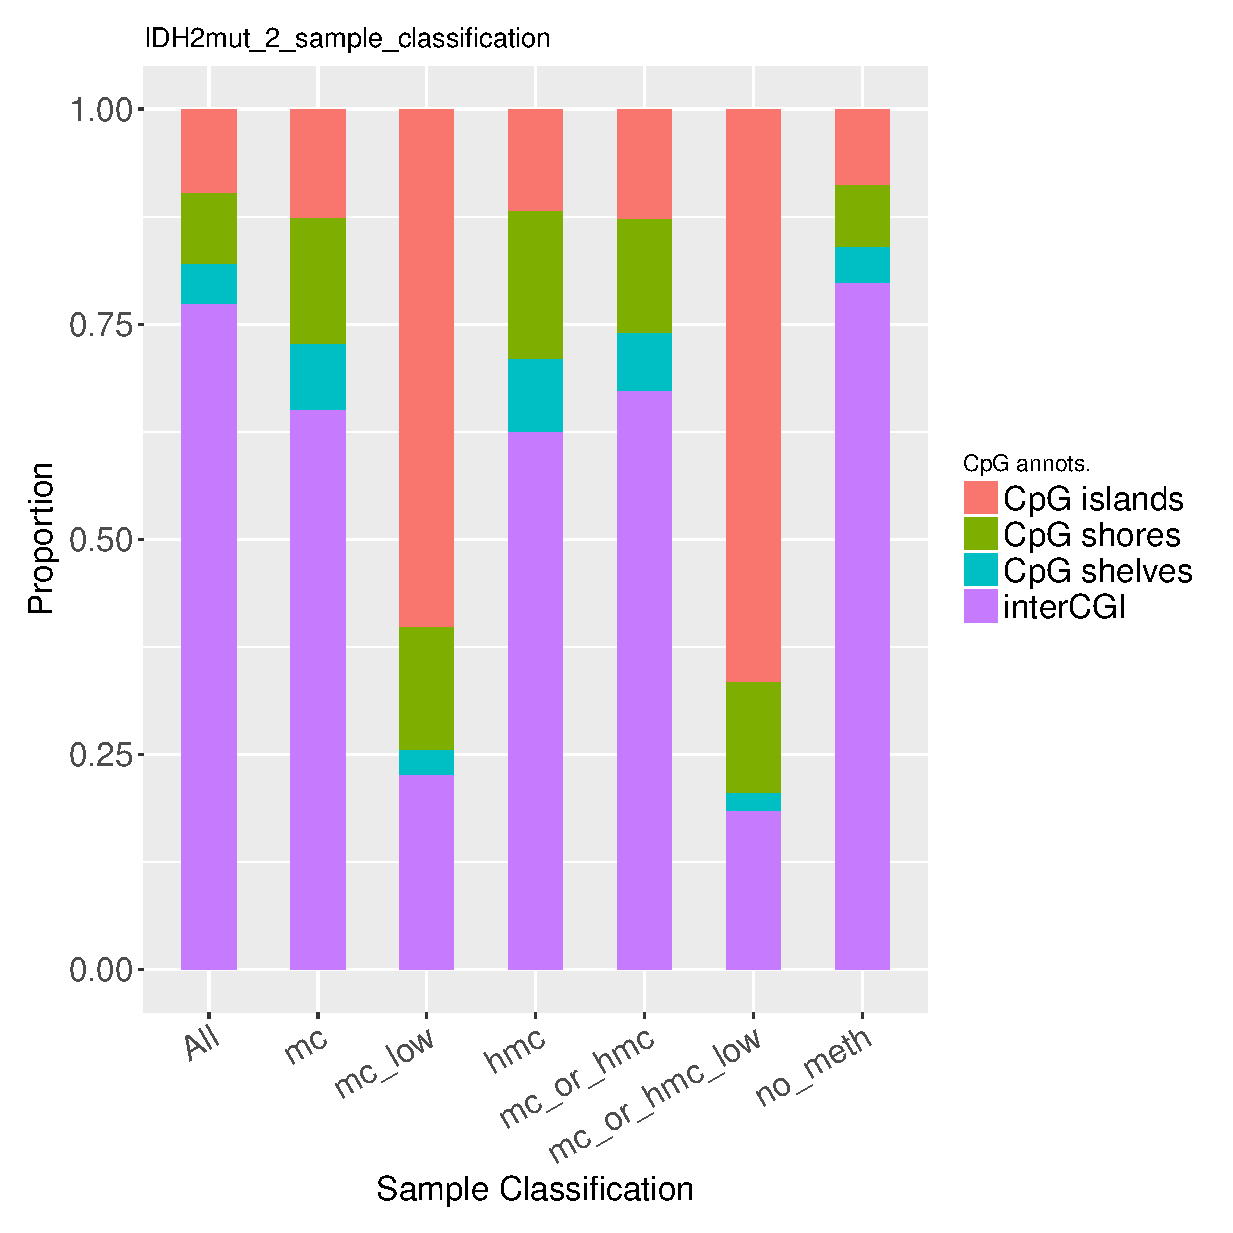
\includegraphics[width=1\textwidth]{chap5figs/figure5_14.eps}
\caption[Genomic annotation to CpG features for sample-wise classification of 5mC and 5hmC signals.]
{
% Rackham requires the figure list title matches the first sentence, so repeat that sentence here
\textbf{Genomic annotation to CpG features for sample-wise classification of 5mC and 5hmC signals.} In the IDH2mut\_2 sample, combined 5mC (mc and mc\_low) classifications occur more frequently in CpG islands (orange) than 5hmC.
}
\label{chap5:fig:14}
\end{figure}

\newpage

\begin{figure}[ht!]
\centering
% manually adjust the width of the figure
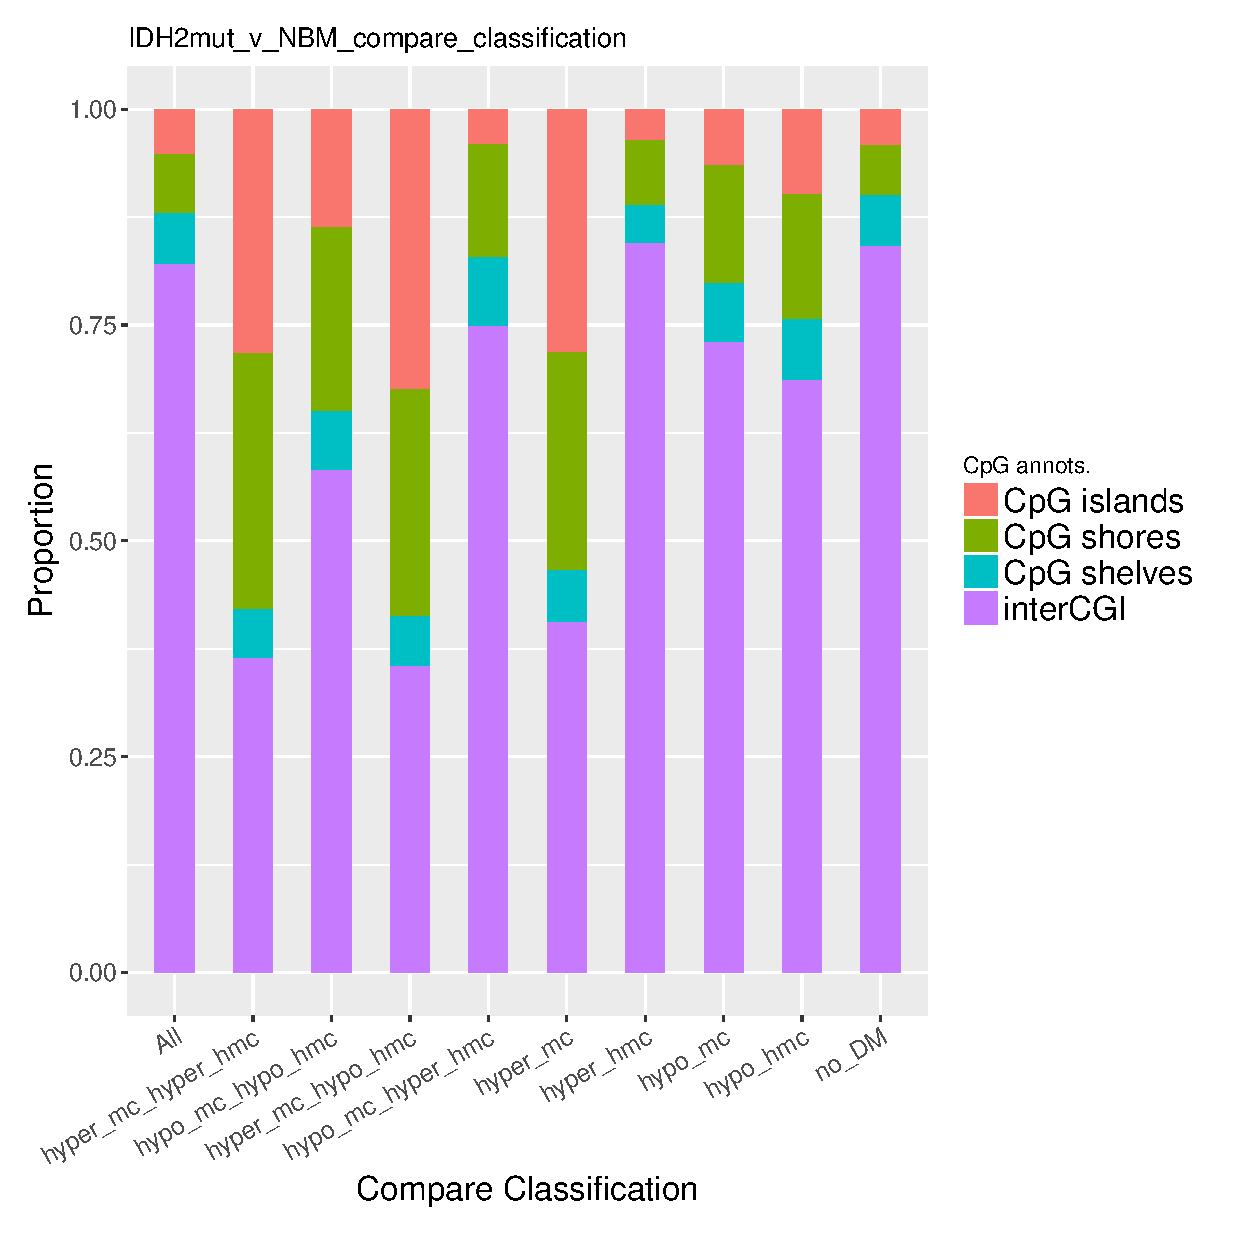
\includegraphics[width=1\textwidth]{chap5figs/figure5_15.eps}
\caption[Genomic annotation to CpG features of DhMR and DMR signal in the comparison of IDH2 mutant to NBM samples.]
{
% Rackham requires the figure list title matches the first sentence, so repeat that sentence here
\textbf{Genomic annotation to CpG features of DhMR and DMR signal in the comparison of IDH2 mutant to NBM samples.}
}
\label{chap5:fig:15}
\end{figure}

\newpage

\begin{figure}[ht!]
\centering
% manually adjust the width of the figure
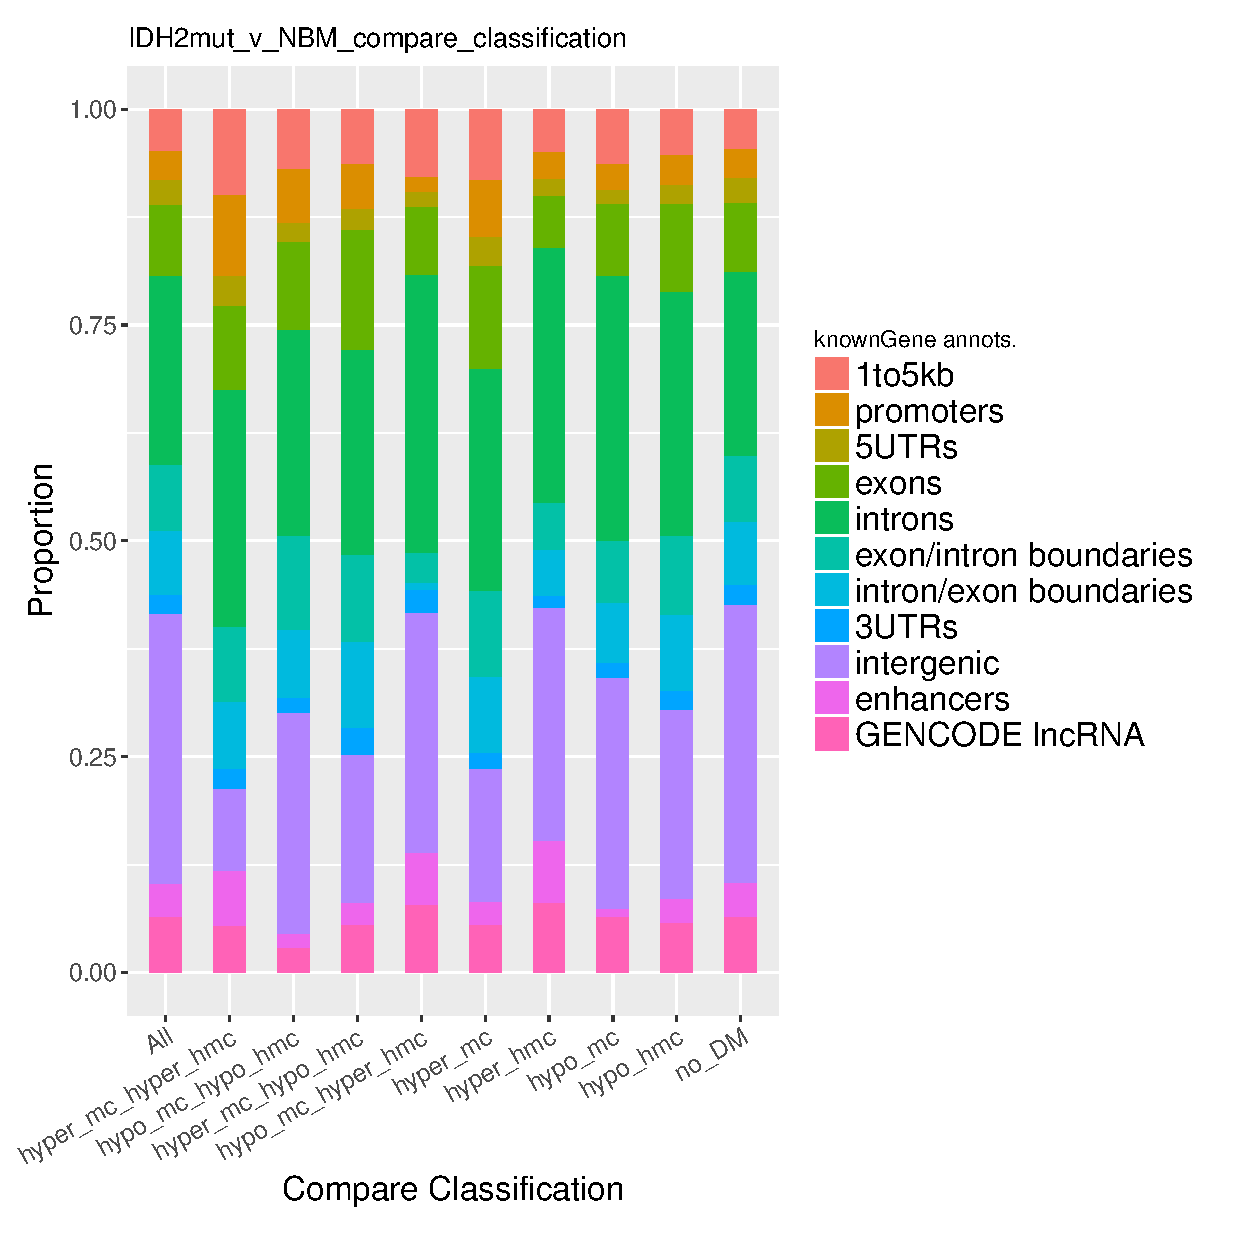
\includegraphics[width=1\textwidth]{chap5figs/figure5_16.eps}
\caption[Genomic annotation to genic features, enhancers, and GENCODE lncRNA of DhMR and DMR signal in the comparison of IDH2 mutant to NBM samples.]
{
% Rackham requires the figure list title matches the first sentence, so repeat that sentence here
\textbf{Genomic annotation to genic features, enhancers, and GENCODE lncRNA of DhMR and DMR signal in the comparison of IDH2 mutant to NBM samples.}
}
\label{chap5:fig:16}
\end{figure}

\newpage

\begin{figure}[ht!]
\centering
% manually adjust the width of the figure
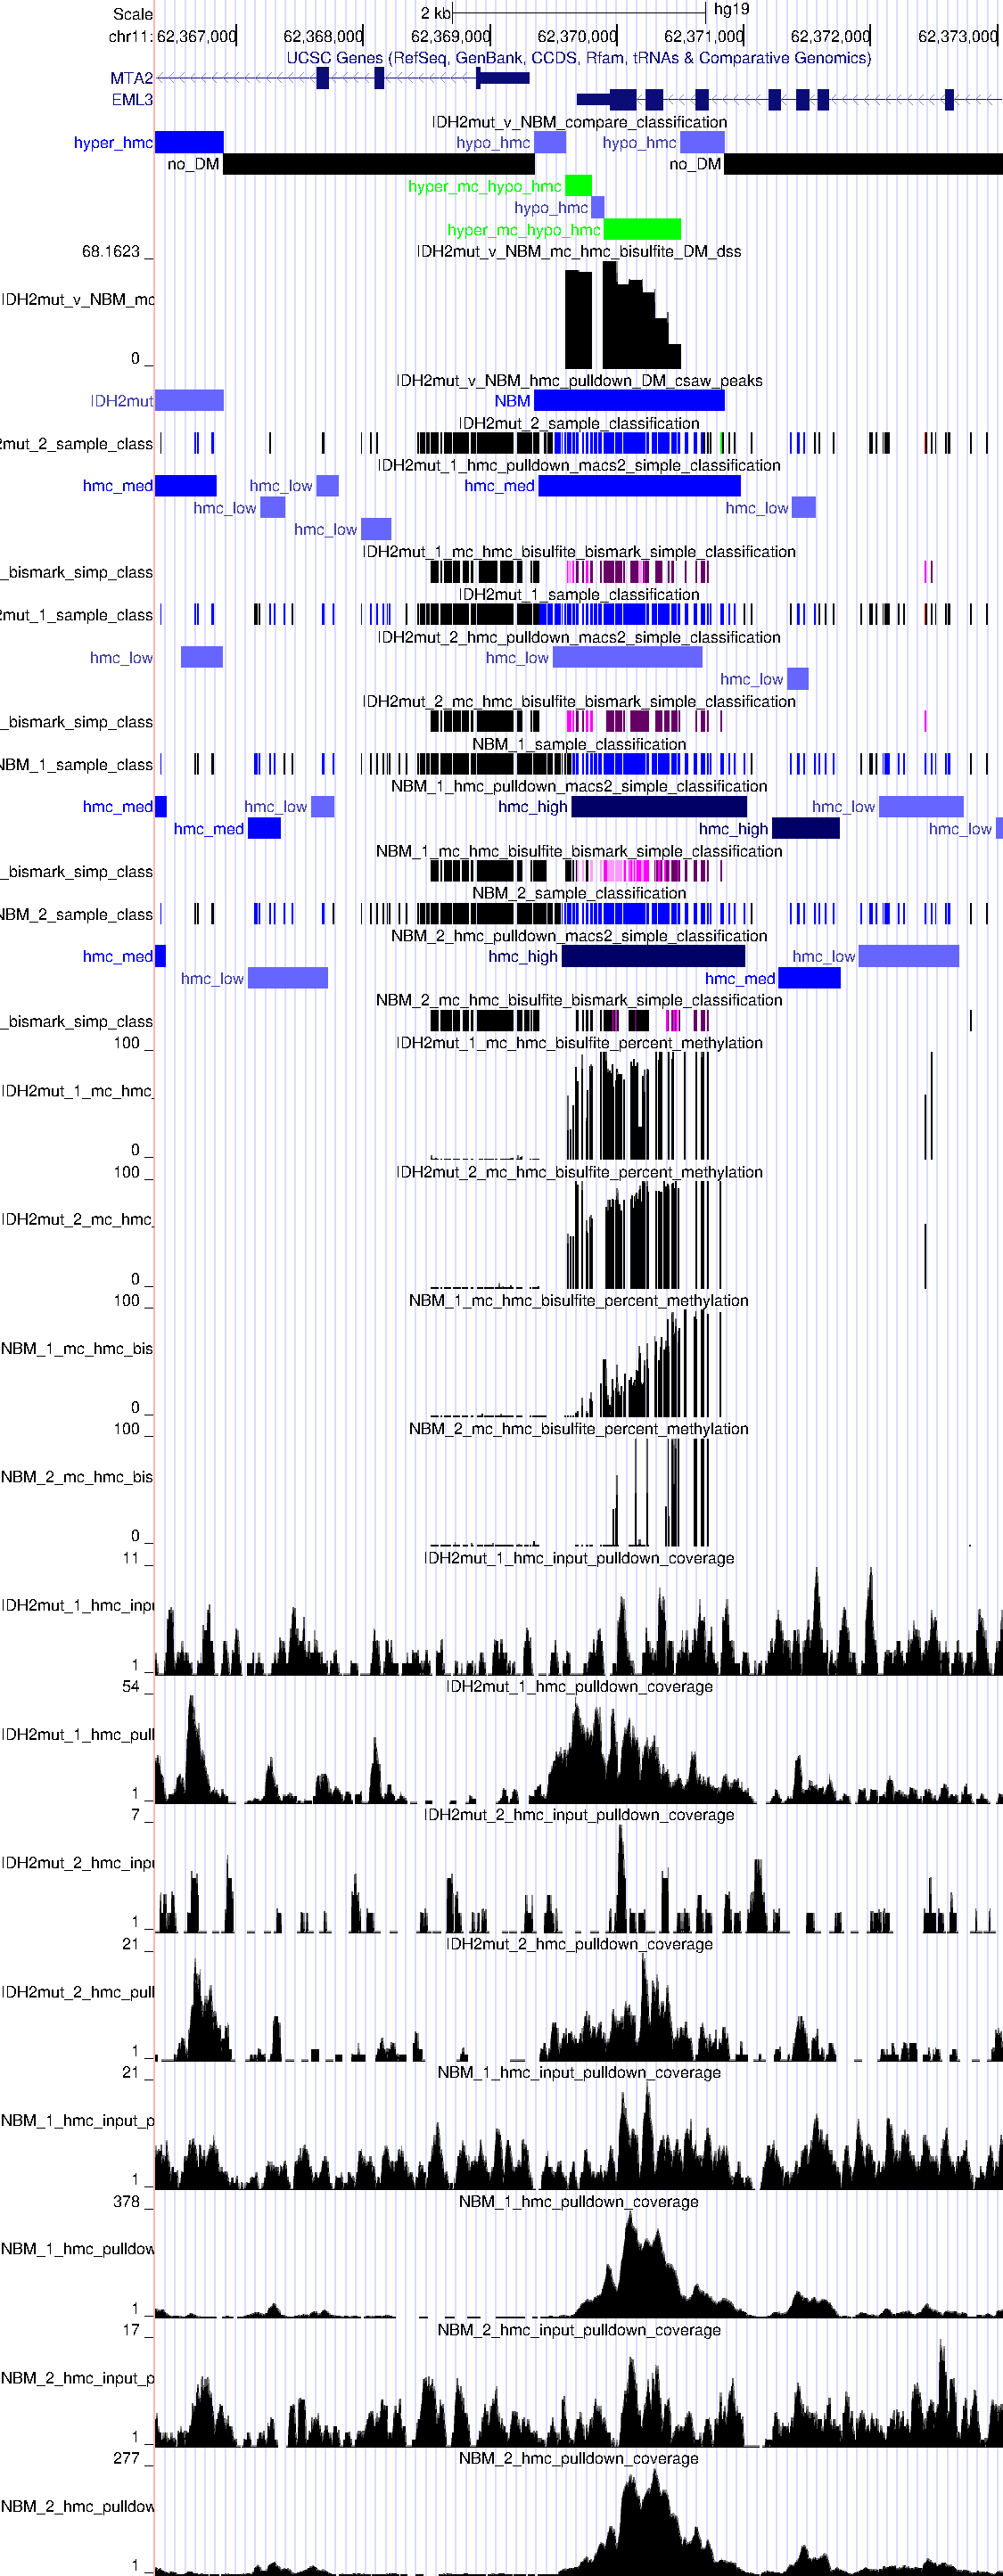
\includegraphics[width=0.5\textwidth]{chap5figs/figure5_17.pdf}
\caption[A display of the entire UCSC Genome Browser track hub.]
{
% Rackham requires the figure list title matches the first sentence, so repeat that sentence here
\textbf{A display of the entire UCSC Genome Browser track hub.} All tracks from the track hub are displayed for the a genomic region containing MTA2 and EML3, which shows simultaneous hypo-hydroxymethylation and hyper-methylation in IDH2 mutants. Tracks have a default grouping based on the track type, but are easily rearranged by the user. For example, the track from the compare\_classification module is grouped with the csaw and DSS tracks since the classification track is the intersection of the latter two.
}
\label{chap5:fig:17}
\end{figure}
